\documentclass[11pt,a4paper]{article}

\usepackage{classeRapport}
\usepackage{minted}
\usemintedstyle{native} %attention l'utilisation de minted n'est pas évidente regarde des tutos si ça bug
%Meilleur mise en page


\begin{document}

\PageDeGarde	
{BoulderDash2.png} % image sur la page de garde
{Rapport de projet I4-2} % titre principal
{Boulder Dash} % sous-titre
{Maxime \textsc{Defromerie}\\
Julie \textsc{Langrand}\\
Victor \textsc{Léger}\\
Romain \textsc{Petitalot}\\
Tom \textsc{Tesniere}} % nom
{I4-2 – STPI2 – 2020-2021} % bas de page


\Page{insa.png} % logo de bas de page (en bas a droite)
\tableofcontents

\clearpage % Pour faire un saut de page propre
\section*{Introduction} % L'astérisque est pour que la section ne soit pas numérotée
\addcontentsline{tod}{section}{Introduction} % Cette commande ajoute la section à la table des matières malgré le fait qu'elle ne soit pas numérotée

    Au cours du semestre 4 de STPI2, nous avons réalisé un projet informatique tout au long du module d'I4-2. Pour ce projet, nous avions le choix entre réaliser soit le jeu Boulder Dash soit le jeu Frogger. Notre choix s'est porté sur le jeu Boulder Dash.
    \paragraph{} Ce projet mêle différentes compétences et il est basé sur l'organisation pour le travail en groupe. Effectivement, nous verrons que l'utilisation de Gitlab a permis de travailler plus facilement sur le projet et tous en même temps. En outre, développer le jeu Boulder Dash a permis de mieux comprendre comment créer un jeu en utilisant la SDL et de renforcer nos compétences en programmation (ici en pascal). La rédaction de ce rapport nous a conduit à utiliser le \LaTeX  afin de séparer le fond de la forme, ce qui est parfait pour un rapport de ce type.


\clearpage % Pour faire un saut de page propre

\section{Analyse du projet}
    Dans cette première partie, nous allons décrire le projet, présenter les fonctionnalités et conceptions que nous avions initialement réalisées. En outre, nous discuterons des éventuelles modifications apportées pour le rendu final.
    
    \subsection{Cahier des charges}
        \subsubsection{Description du projet}
        Le groupe a décidé de faire un Boulder Dash, car nous y avions déjà tous joué avant ce projet. De plus, les graphismes sont agréables et le jeu est relativement addictif. Ainsi, notre choix s'est rapidement tourné vers ce dernier et les idées de conception du jeu ont été rapides. 
        \\
        \\
        Boulder Dash est un jeu où l'on incarne un petit personnage dont le but est de ramasser des diamants en creusant la terre. 
        Ce jeu possède différents niveaux dont la difficulté est progressive. Dans ces niveaux, on retrouve des ennemis et des rochers. 
        Le joueur possède 3 vies, si le joueur se fait écraser par un rocher ou toucher par un ennemi, il perd une vie, au bout de 3 vies perdues la partie du joueur est terminée. Certains niveaux ne possèdent pas de diamants, le joueur doit alors tuer les ennemis du niveau en faisant tomber un rocher sur eux ce qui fera apparaître des diamants. Les diamants peuvent aussi tomber sur d'autres ennemis les tuant à leur tour. Le joueur peut aussi casser des murs pour atteindre des zones bloquées grâce aux rochers.
        Nous avons aussi la volonté d’ajouter des fonctionnalités facultatives telles que la création de niveau par l’utilisateur ou encore la personnalisation du personnage jouable (ces fonctionnalités sont listées dans la partie suivante).

        \subsubsection{Liste des fonctionnalités}\label{sssect:fonctionnalites}
            Le rendu final de notre projet doit comporter les fonctionnalités suivantes:
            \vspace{0.2cm}
            \begin{itemize}
                \item Déplacement du joueur 
                \item Chargement des niveaux (mur, terre, bords, rochers) depuis un fichier .txt
                \item Sauvegarde de la partie 
                \item Différents niveaux
                \item Menu
                \item Victoire (débloquer passage pour terminer niveau)
                \item Détection de mort (écrasé par un rocher, touché par un ennemi) 
            \end{itemize}
            \vspace{0.3cm}
            Nous avons prévu des fonctionnalités optionnelles, afin d'améliorer le jeu, que nous ferions si le temps le permettait :
            \vspace{0.2cm}
            \begin{itemize}
                \item Création de niveaux par l’utilisateur
                \item Musique 
                \item Personnalisation joueur
                \item Ajout d’ennemi  et/ou de PNJ
                \item Choix mondes
                \item Chronomètre 
                \item Animation mort personnage (si écrasé par un rocher ou touché par un ennemi)
            \end{itemize}
            
            \vspace{0.3cm}
            \textbf{Versions prévues:}
            
            V1 (08/04/2021):
            \begin{itemize}
                \item Déplacement du joueur
                \item Chargement de niveaux depuis des fichiers .txt 
            \end{itemize}
            \vspace{0.2cm}
            
            V2(22/04/2021):
            \begin{itemize}
               \item Mise en place de différents niveaux
               \item Sauvegarde de la partie
               \item Implémentation du menu
                \item Mise en place de la détection de mort
            \end{itemize}
            \vspace{0.2cm}
            
            V2(07/06/2021):
            \begin{itemize}
               \item Finalisation des fonctionnalités présentes
               \item Implémentation des fonctionnalités facultatives
               
            \end{itemize}



    \subsection{Conception globale}
        Cette section présente la conception globale de notre programme implémentant les fonctionnalités données en section~\ref{sssect:fonctionnalites}.
        L'analyse descendante correspondante est donnée à la page suivante.
        
        \newpage
        
        Voici l'analyse descendante intiale de notre projet :
        \vspace{0.3cm}
        
        \rotatebox{90}{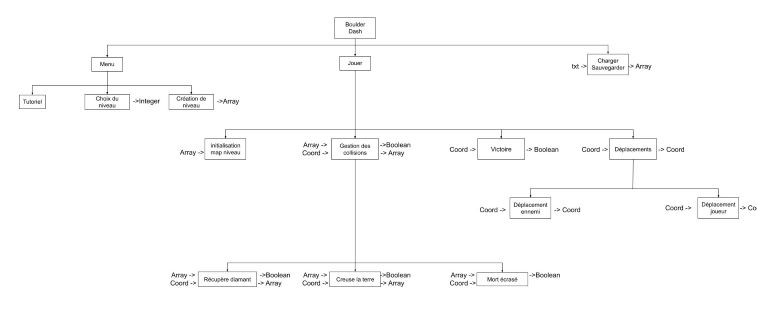
\includegraphics[width=190mm]{images/AD-T.jpg}}
        
        Cette analyse descendante a été relativement bien suivie. Cependant, nous avons tout de même changé quelque peu cette dernière. Les principales modifications sont les suivantes : 
        \\
        \begin{itemize}
            \item changement n°1 :
            Un des changements notable est l'implémentation de différentes unités. Une première unité ("rockfordUtils.pas") a été utilisée pour stocker les différentes structures utilisées tout au long du programme principal. Une seconde unité ("menurockford") a été implémentée permettant de bien séparer le jeu principal du menu et donc de simplifier l'écriture du code pour ces deux parties.
            \\
            \item changement n°2 :
            On peut noter de plus que certaines entrées et sorties ont été modifiées et de nouvelles ont été rajoutées, n'apparaissant pas dans l'analyse descendante, du fait de l'adaptation de notre programme au langage de programmation SDL.
            \\
        
        \end{itemize}
    
    \newpage
    \subsection{Conception préliminaire}
        Le contenu de cette section présente la signature des fonctions et procédures de notre analyse descendante, en précisant les entrées, sorties et entrées/sorties.
        
        \begin{algorithm}
            \begin{algorithmic}
                \Procedure{Jouer}{ }
                \vspace{0.2cm}
                \Procedure{GestionCollisions}{E c : Coord, E/S t : Tab, S Coli: booleen}
                \vspace{0.15cm}
                \Function{MortEcrase}{t : Tab, c : Coord} : Booléen
                \EndFunction
                \Procedure{RecupereDiamant }{E c : Coord, E/S t : Tab, S Dia : Booléen }
                \EndProcedure
                \Procedure{CreuseTerre}{E c : Coord, E/S t : Tab, S Terre: Booléen }
                \vspace{0.2cm}
                \EndProcedure
                \EndProcedure
                \Function{victoire}{c : Coord} : Booléen
                \vspace{0.2cm}
                \EndFunction
                \Procedure{Deplacement}{ E/S c : Coord}
                \vspace{0.15cm}
                \Procedure{DeplacementJoueur}{E/S cPlayer : Coord}
                
                \EndProcedure
                \Procedure{DeplacementEnnemi}{E/S cEnnemy : Coord}
                
                \EndProcedure
                
                \EndProcedure
                \vspace{0.2cm}
                \Procedure{InitMapNiveau}{E t : tab}
                \vspace{0.2cm}
                
                \EndProcedure
                \EndProcedure
                \Procedure{ChargerSauvegarder}{E f : txt, S t : Tab}
                \EndProcedure
                \vspace{0.2cm}
                \Procedure{Menu}{ }
                \vspace{0.15cm}
                \Procedure{Tutoriel}{ }
                \EndProcedure
                \Procedure{ChoixNiveau}{}
                \EndProcedure
                \Procedure{CreationNiveau}{t : Tab}
                \EndProcedure
                
                \EndProcedure
            \end{algorithmic}
        \end{algorithm}
        
        A nouveau, quelques changements ont eu lieu en pratique : 
        \begin{itemize}
            \item changement n°1 : La procédure tutoriel n'a pas été réalisée compte tenu de la simplicité du jeu, la procédure CreationNiveau n'a pas été implémentée dans notre code, car ce n'était pas pertinent pour notre jeu et nous avons préféré nous focaliser sur des aspects plus importants du jeu.
            \item changement n°2 La procédure RecupererDiamant a été directement mise dans celle du déplacement du joueur car c'était plus simple à coder.
            \item changement n°3 Comme cité précédemment, l'utilisation de la bibliothèque SDL nous a contraint à modifier les entrées et sorties de chacune des procédures et fonctions.
        \end{itemize}
        
        
        De plus, nous avons utilisé de nombreux types structurés dans notre projet, à commencer par les coordonnées du Menu (coordMenu), les coordonnées du joueur (coordonnees) mais aussi un type block pour définir le tableau de structures Terrain qui était un composé de block pour représenter la grille de jeu.
        
        
        
        
        
        
        
    \subsection{Procédures ou fonctions importantes}
       Les deux procédures que nous avons retenues sont :
       \\
       \\
       - La procédure "chargement"
       \\
       \\
       - La procédure "tombePierre"
        \\
        \\
        Ces deux procédures nous semblaient pertinentes, car elles sont nécessaires au bon fonctionnement de notre programme et leur implémentation s'est avérée quelquefois plus complexe que l'on pensait.
        \\
        \\
        La difficulté principale dans la procédure chargement était de charger toutes les données du niveau notamment la position du personnage, de l'arrivée, et l'ensemble des objets du niveau. De plus, la procédure SauvegarderNiveau devait être complémentaire à cette procédure pour charger des fichiers sauvegardés et se souvenir, par exemple, du nombre de diamant déjà récupérés ou du temps écoulé.
        Quant à la procédure tombePierre, la difficulté résidait dans le fait de gérer tous les types d'éboulements (par le bas et les côtés) pour les pierres et les diamants et les différents délais d'affichage pour chacun des mouvements et également les collisions avec notre personnage et les PNJ. 
        \\
        \\
\newpage

\begin{minted}
[
frame=lines,
framesep=2mm,
baselinestretch=1.2,
bgcolor=black!75,	
fontsize=\footnotesize,
linenos
]
{pascal}
//Procedure chargement du terrain de jeu
procedure chargement (name : string; var T : Terrain;var posRF, posFin : coordonnees;var 
nbDiamant, nbDiamantFin, reserveTemps : Integer);
var fic	:Text;
	i, j : Integer;
	str: String;
begin
	assign(fic,name + '.txt');
	reset(fic);
	i:=1;
	read(fic, posRF.x);//On commence par lire les données du niveau
	readln(fic, posRF.y);
	read(fic, posFin.x);
	readln(fic, posFin.y);
	read(fic, nbDiamant);
	readln(fic, nbDiamantFin);
	readln(fic, reserveTemps);
	while (not eof(fic)) do
	begin
		readln(fic,str);
		for j := 1 to 24 do
		begin
			T[i][j].genre := StrToInt(str[j]);//On lit la map
			T[i][j].mouvement := '';
		end;
		i:=i+1;	
	end;
	close(fic);
	T[posRF.y][posRF.x].genre := 0;//Notre personnage part sur une case vide
	initPapillon(T);//Calcul de la direction dans laquelle les papillons vont devoir partir
end;
\end{minted}
        
\newpage

\begin{minted}
[
frame=lines,
framesep=2mm,
baselinestretch=1.1,
bgcolor=black!75,	
fontsize=\footnotesize,
linenos
]
{pascal}
//Procedure tombePierre permettant la chute de la pierre
procedure tombePierre(var window, rockford : Psdl_Surface; var T:Terrain; position : coordonnees;
nomObjet:string; var nbDiamant : Integer; var fin : Boolean );
var i, j, numeroObj, coordY : Integer;
begin
	if nomObjet = 'Pierre' then
		numeroObj := 3
	else if nomObjet = 'Diamant' then
		numeroObj := 4;
	
	for i := 1 to largueur do
	begin
		for j := 1 to longueur do
		begin
			if T[i][j].mouvement = nomObjet then
			begin
				T[i+1][j].genre := numeroObj;
				T[i][j].mouvement := '';
				afficherfond(window, rockford, T, position, True);
				if (position.y = i+2) and (position.x = j) then 
					fin := True;
				if T[i+2][j].genre = 6 then
				begin
					mortPapillon(T, j,i+1, nbDiamant, position);
					mortPapillon(T, j,i+2, nbDiamant, position);
					mortPapillon(T, j,i+3, nbDiamant, position);
				end;
			end;
			if T[i][j].genre = numeroObj then
			begin
				if (T[i+1][j].genre = 0) and not((position.y = i+1) and 
				(position.x = j)) then
				begin
					T[i][j].genre := 0;
					T[i][j].mouvement := nomObjet;
					afficherfond(window, rockford, T, position, True);
					SDL_Flip(window);
				end
				else if (T[i+1][j].genre = 6)then
				begin
					mortPapillon(T, j,i, nbDiamant, position);
					mortPapillon(T, j,i+1, nbDiamant, position);
					mortPapillon(T, j,i+2, nbDiamant, position);
				end;
			end;					
			if T[i][j].genre = numeroObj then //Les éboulements sur le côté
			begin
				if (T[i+1][j].genre = 3) or (T[i+1][j].genre = 4) then
				begin
					coordY := i+1;
					while (T[coordY][j].genre = 3)or(T[coordY][j].genre = 4) do
					//Pour verif que la pierre en dessous ne tombe pas
					begin
						coordY := coordY +1;					
					end;
					if T[coordY][j].genre <> 0 then
					begin
						if (T[i+1][j+1].genre=0)and(T[i][j+1].genre=0)and
						not((position.y=i+1)and(position.x=j+1))and
                        not((position.y=i)and(position.x=j+1))
                        and(T[i][j+1].mouvement='')then
						begin
							T[i][j+1].genre := numeroObj;
							T[i][j].genre := 0;
							afficherfond(window,rockford,T,position,True);
							SDl_delay(50);
							T[i][j+1].genre := 0;
							T[i+1][j+1].genre := numeroObj;
						end
						else if(T[i+1][j-1].genre=0)and(T[i][j-1].genre=0)and
						not((position.y=i+1)and(position.x=j-1))and
					    not((position.y=i)and(position.x=j-1))
					    and(T[i][j-1].mouvement='')then
						begin
							T[i][j-1].genre := numeroObj;
							T[i][j].genre := 0;
							afficherfond(window,rockford,T,position,True);
							SDl_delay(50);
							T[i][j-1].genre := 0;
							T[i+1][j-1].genre := numeroObj;
						end;
					end;
				end;
			end;
		end;
	end;
	afficherfond(window, rockford, T, position, True);
end;
\end{minted}
        
\newpage
   
    \subsection{Partie développement}
        \subsubsection{Les unités et le programme principal}
            \begin{itemize}
                \item {Unité rockfordUtils} : Cette unité comprend toutes les différentes constantes et les différents types utilisés dans notre projet. Pour les constantes, on y retrouve par exemple la largeur et la longueur de la fenêtre de jeu. Pour les différentes unités, nous avons notamment les coordonnées du joueur en x et y, les coordonnées du menu en x et y, mais aussi avec une variable représentant le choix du joueur dans le menu. Puis un tableau Terrain composé du type "block" qui représente les différentes cases de notre jeu.
                \\
                \item {Unité menurockford} : Cette unité est composée de plusieurs procédures d'affichages des différentes parties du menu, avec le fond mais aussi le curseur (représenté par le personnage rockford), d'une procédure pour la gestion du clavier de l'utilisateur et deux procédures pour gérer le son. Toutes ces procédures sont regroupées dans la procédure menu qui les combine. La procédure menu est ensuite utilisée dans le code principal du jeu. On peut également citer les deux dernières procédures : ProcessKeyFin et choixFin qui permettent de quitter le jeu en le sauvegardant ou non.
                \\
                \item {Programme principal} : Le programme principal du jeu qui regroupe toutes les procédures de gestion du jeu, celles liées aux déplacements du joueur, des ennemis ou des pierres mais aussi des procédures d'affichages de tous les blocs et celle pour le temps de jeu. Puis, nous avons les procédures pour sauvegarder et charger le jeu à partir de fichier texte qui se situe dans un dossier intitulé "Ressources". Le code principal initialise les variables, reprend le menu puis charge le jeu. Ensuite, le jeu se fait grâce à une itération sur le déplacement du joueur et des ennemis. Enfin, suivant le choix du joueur, si ce dernier meurt ou gagne, le jeu s'arrête. En outre, s'il appuie sur échap en pleine partie, il peut choisir de sauvegarder le jeu ou de reprendre la partie.
            \end{itemize}
        
        \subsubsection{Utilisation de la SDL}
        La bibliothèque SDL était essentielle pour notre projet. En effet la gestion du clavier et l'affichage vidéo permettent au joueur d'avoir une meilleure expérience que sur une version avec un terminal. Néanmoins les procédures et fonctions ont toutes été pensées au début sans SDL, ce n'est que pendant le développement et l'écriture du code sur Pascal que nous avons rajouté les éléments liés à la SDL dans notre code. 
        
 

\section{Exemple de section}

    \subsection{Comment apprendre le \LaTeX}
        L'usage du \LaTeX{} peut être déroutant au début (cf. figure~\ref{chien}), cette approche de la composition de document étant très loin de ce que l'on fait lorsque l'on utilise des logiciels comme Microcrotte Office ou Libre Office.
        Sans rentrer dans les détails, il faut voir le \LaTeX{} comme un outil permettant de séparer \emph{le fond} (ce que vous allez mettre dans votre document), de \emph{la forme} (comment le fond va apparaître dans le document final).

        \begin{figure}[!ht]
            \centering % Centre horizontalement tout ce qui est dans l'environnement ``figure''
                
\includegraphics[width=0.5\textwidth]{images/tech-support-dog.jpg} % Chemin vers l'image à ajouter
            \caption{Toi en train d'apprendre le \LaTeX.} % Légende de l'image
            \label{chien} % Étiquette pour y faire référence ailleurs dans le document
        \end{figure}
        
        Quand vous écrivez du code \LaTeX, vous vous contentez en grande majorité de décrire le fond:
        je veux un paragraphe qui contient ce texte (on sépare deux paragraphe de texte par une ligne vide), je commence une nouvelle section/sous-section/sous-sous-section ici (en utilisant la commande \verb|\section{}|/\verb|\subsection{}|/\verb|\subsubsection{}|), je veux mettre en valeur \emph{cette partie de phrase} (en utilisant la commande \verb|\emph{}|)…
        La forme est gérée plus tard, par un modèle de document par défaut que vous pouvez éventuellement modifier indépendamment du fond.

        La meilleure manière d'apprendre à coder en \LaTeX{} est \emph{de bricoler du code \LaTeX{} et de voir ce qu'il se passe.}

        \subsubsection{Quelques bonnes pratiques}
            Je donne ici quelques lignes directrices qui, si elles sont respectées, vous éviteront un certain nombre de difficultés lors de l'écriture d'un document \LaTeX{}.
        
            \paragraph{Bien organiser son code source}
                Écrire du \LaTeX{}, c'est écrire du \emph{code source}.
                Comme vous l'avez appris à l'INSA, un bon code source doit être proprement mis en forme.
                Je vous recommande, lorsque vous écrivez du texte, d'écrire une phrase par ligne, cela rendra votre code bien plus lisible et simplifiera l'utilisation d'un logiciel de gestion de sources comme git.
                En ce qui concerne la lisibilité du code source, pensez à \emph{indenter} votre code afin de mieux vous y repérer.
            
             \paragraph{Compiler du \LaTeX{}}
                Étant donné que le \LaTeX{} est du code source, celui-ci doit être compilé (à l'aide de la commande \verb|pdflatex| par exemple).
                Comme pour un programme en Pascal, à la compilation il est possible que des messages d'avertissement ou d'erreur s'affichent.
                La plupart des messages d'avertissement ne posent pas de problèmes (le document que vous lisez en émet un certain nombre à la compilation), cependant les messages d'erreur sont beaucoup plus graves et doivent être résolus pour obtenir un document final correct et complet.
                Ce n'est pas par ce qu'à la fin de votre compilation vous obtenez un document que la compilation s'est passée sans erreur.
                Dans la plupart des cas, aucun document n'est produit, mais certains éditeurs de \LaTeX{} \enquote{forcent} la compilation jusqu'au bout.
                Je vous invite donc à être très attentif à comment se déroule la compilation de votre document de manière à ne pas passer à côté d'erreurs de compilation.
                Je vous invite aussi à \emph{compiler votre document aussi souvent que possible}, cela afin de repérer le plus tôt possible les erreurs de compilation dans le code source que vous tapez.
        
        \subsubsection{Ressources externes}\label{sssect:ressources_externes}
            Pour vous aider dans votre aventure d'écriture de beaux documents, voici quelques ressources sur lesquelles vous pouvez vous appuyer pour rechercher de l'information.
            Je vous recommande d'y avoir recours quand le besoin s'en fait ressentir lorsque vous rédigez votre document.
            
            \paragraph{Wikilivres}
                Les wikilivres sur le \LaTeX{} (en français et en anglais) sont particulièrement bien rédigés et traitent un grand nombre de cas de figure face auxquels on peu se retrouver:
                \begin{itemize}
                \item En français: \url{https://fr.wikibooks.org/wiki/LaTeX}
                \item En anglais: \url{https://en.wikibooks.org/wiki/LaTeX}
                \item Le vadémécum du livre français vaut le détour: \url{https://fr.wikibooks.org/wiki/LaTeX/Vad%C3%A9m%C3%A9cum}
                \end{itemize}
            
            \paragraph{\LaTeX{} stack exchange}
                Le site internet \url{https://tex.stackexchange.com/} est un espace dédié aux questions/réponses sur la thématique du \LaTeX{}.
                Les réponses y sont souvent correctes et bien documentées (mais pas toujours! Faites preuve de recul.).
                Les sujets abordés varient grandement en termes de complexité, à vous de vous y retrouver.
                
                Petite mise en garde en passant: vous copiez-collez du code depuis internet \emph{à vos risques et périls}.
                Si vous ne comprenez les commandes que vous utilisez dans votre code, vous ne comprendrez pas les erreurs que celui-ci produit.
                Ce n'est pas par ce qu'une personne, sur internet, à une moment donné, à proposé une idée pour faire une chose que cette idée est la bonne pour faire ce que vous voulez.
            
            \paragraph{Le Comprehensive \TeX{} Archive Network}
                Pour les braves.
                Si vous souhaitez comprendre dans le détail comment un paquet \LaTeX{} fonctionne et comment l'utiliser, vous trouverez sa documentation sur le site \url{https://www.ctan.org/}.
                C'est souvent très instructif mais il faut être un minimum à l'aise avec le \LaTeX{} pour se plonger dans ce type de documentation.




    \subsection{Comment ne pas apprendre le \LaTeX}
        Comme dit précédemment, l'apprentissage du \LaTeX{} se fait par la \emph{pratique}.
        Essayer d'apprendre à utiliser ce langage en parcourant uniquement les références données dans la section~\ref{sssect:ressources_externes} sans jamais s'aventurer à écrire du code ne vous apportera rien.
        
        Si à un moment vous êtes bloquez et n'arrivez pas à vous en sortir même avec l'aide de vos camarades, vous pouvez solliciter de l'aide soit auprès d'un enseignant en TP, soit éventuellement sur internet.
        Soyez conscient que le code que vous avez écrit \emph{vous appartient}.
        Vous en êtes responsables.
        Si vous demandez un appui extérieur, assurez-vous de montrer que vous avez cherché à comprendre et résoudre le problème par vous-même.
        Envoyer par mail ou sur un forum un code source qui ne compile pas en demandant à ce que votre interlocuteur le répare à votre place est le meilleur moyen de vous le mettre à dos et de recevoir un lapin pancake comme réponse (cf. figure~\ref{lapin}).
        
        
        \begin{figure}[!ht]
            \centering % Centre horizontalement tout ce qui est dans l'environnement ``figure''
                
\includegraphics[width=0.5\textwidth]{images/pancake-bunny.jpg} % Chemin vers l'image à ajouter
            \caption{Ma réponse quand on me pose une question sur du \LaTeX{} sans avoir essayé de chercher une solution par soi-même.} % Légende de l'image
            \label{lapin} % Étiquette pour y faire référence ailleurs dans le document
        \end{figure}


\clearpage % Pour faire un saut de page propre

\section{Conclusion}

    Pour conclure, ce projet d'I4-2 nous a permis de développer de nombreuses compétences et fut une expérience enrichissante pour l'ensemble du groupe. Néanmoins, nous avons rencontré plusieurs difficultés au cours de notre projet. En effet, le travail à distance empêchait une bonne cohésion d'équipe et cela a été difficile de se coordonner au début du projet. Par la suite, pour le code, certains avaient déjà coder en SDL, c'est pourquoi ils ont aidé les personnes qui avaient plus de mal avec cette bibliothèque. 
    Au cours de ce projet, nous avons eu l'occasion de développer notre expérience dans le travail de groupe qui est une des compétences majeures d'un ingénieur aujourd'hui. De plus, nous avons renforcé nos connaissances et compétences en programmation avec l'utilisation du langage de programmation SDL et Pascal. L'utilisation des bibliothèques SDL fut une première approche pour certains et pour d'autres a permis l'approfondissement de leurs compétences. Enfin l'utilisation de nouveaux outils tels que Gitlab ou encore l'écriture du rapport en \LaTeX a permis à l'ensemble du groupe la maîtrise d'outils s'avérant nécessaire pour la suite de notre cursus.


\clearpage % Pour faire un saut de page propre

\section*{Sources} % L'astérisque est pour que la section ne soit pas numérotée
\addcontentsline{toc}{section}{Sources} % Cette commande ajoute la section à la table des matières malgré le fait qu'elle ne soit pas numérotée
    \begin{itemize}
        \item Photo de la page de garde: \url{http://emultest.free.fr/screenshot/nes/boulderdash1.png}
    \end{itemize}




\end{document}
